
\subsection{Intracellular recordings}
\label{Lymnaea stagnalis preparation}
The experimental data was obtained using intracellular electrophysiological recordings with sharp electrodes in the neurons of \textit{Lymnaea stagnalis}. This animal model was used because of the easy accessibility of the neurons that are distributed and organized in different ganglia, with a distinct function associated to each one of them. For the experiments, we chose the right parietal ganglion since it is one of the largest ganglia in the system and so are its neurons. In addition, many neurons in this ganglion are usually spontaneously active and present a tonic spiking that can last for hours. It is also convenient of this animal that its neural activity is slow, which allows us to explore the modulation of the action potential dynamics at multiple time scales with larger resolution in the electrophysiological recordings. Membrane potential was recorded using 3 M $KCl$ filled electrodes and a DC amplifier (ELC-03M, NPI Electronic, Hauptstrasse, Tamm, Germany). Recordings were acquired at 10 KHz using an A/D board (PCI-625 with a BNC-2090A DAQ device, National Instruments). 

\subsection{\textit{Lymnaea stagnalis} preparation}

The neural system was isolated from the rest of the body to perform the electrophysiological recordings. The body shell was removed, along with other visceral parts above the neural system. Then, all nerves attaching the system to the body and the buccal ganglia to the buccal mass were cut, so the system was isolated (see Fig. \ref{fig:methods_general}A). The preparation was immersed in a saline solution (in mM: 51.3 $NaCl$, 1.7 $KCl$, 1.5 $MgCl_2\cdot6H_2O$, 4.1 $CaCl_2\cdot2H_2O$, 5 $HEPES$, corrected to pH 7.8 with 4 $M$ $NaOH$).
The sheath above the ganglia that restricts the access to the neuron with the sharp electrode was reduced using \textit{Protease} (Sigma type XIV). All procedures followed the European Commission and Universidad Autónoma de Madrid animal treatment guidelines.

\subsection{Spike waveform characterization parameters} \label{sec:characterization parameters}
\label{sect:metrics}
% Data analysis was performed in Python 3.8. 
For both experimental recordings and model simulations, action potentials were detected as the max point over a threshold, and each waveform was segmented 100ms before and after the peak temporal reference. For the superposition of action potentials (Figs. \ref{fig:continuous_results_panel},\ref{fig:continuous_model},\ref{fig:temperature model},\ref{fig:q10 dependency}) the waveforms were aligned in the x-axis by the peak and in the y-axis by the first point of the waveform voltage values.

For the waveform shape characterization, we used four different parameters: duration, amplitude, depolarization and repolarization slopes. They are depicted in Fig. \ref{fig:methods_general}B and defined as follows:
\begin{itemize}
    \item Duration: Time interval between the two points at half width of the action potential. 
    \item Amplitude: Difference between minimum and maximum voltage values in the waveform. 
    \item Depolarization slope: Slope in the depolarization phase measured 10 points before and after the half width point reference before the peak.
    \item Repolarization slope: Slope in the depolarization phase measured 10 points before and after the half width point reference after the peak.
\end{itemize}

To compare recordings from different neurons and between model simulations and experimental data, we normalized the change between the laser and the control for each metric using the following expressions for electrophysiological data and model simulations, respectively:
\begin{equation}
    {metric\ change}_{experimental} = \frac{|metric_{laser} - metric_{control}|}{|mean(metric_{control})|},
\end{equation}

\begin{equation}
    {metric\ change}_{model} = \frac{|metric_{min} - metric_{max}|}{|metric_{max}|}.
\end{equation}

All data analysis was performed in Python, the scripts are available in \href{https://github.com/GNB-UAM/Garrido-Pena_Modulation-neural-dynamics-by-CW-NIR-stimulation}{github.com/GNB-UAM/\\Garrido-Pena\_Modulation-neural-dynamics-by-CW-NIR-stimulation}.

\begin{figure}[htb!]
    \centering
    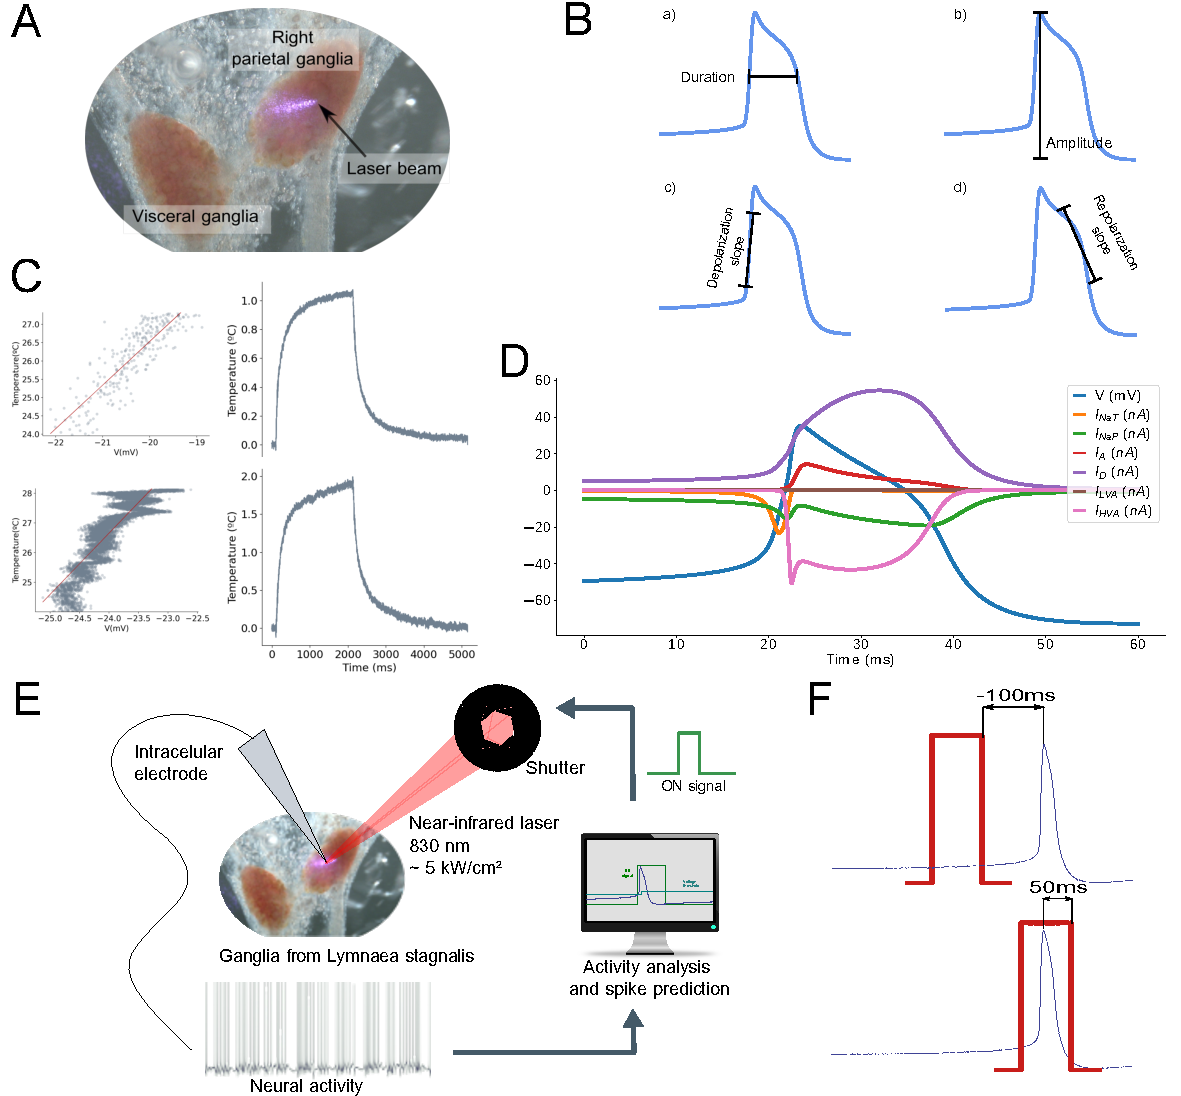
\includegraphics[width=\textwidth]{images/methods/Fig1_methods_general_w_temperature_estimation.pdf}
    \caption{A. Illustration of the laser beam focused on a neuron in the right parietal ganglia at maximum power showing a sharpened form due to the angle. B. Representation of waveform shape's metrics: a) Spike duration at half width. b) Spike amplitude between the maximum and minimum voltage values. c) Depolarization slope at half width. d) Repolarization slope at half width. C. Open-pipette temperature estimation method. Left column, temperature and voltage relation. Second column filtered mean of voltage recordings from short illumination intervals in the pipette. D. Simulation of the CGC-model representing the voltage dynamics during an action potential and the corresponding ionic currents defined in the model ($I_{NaP}$, $I_{INaT}$, $I_A$, $I_D$, $I_{LVA}$, $I_{HVA}$). The units in the y-axis (in relative values) are defined in the legend, respectively. E. Activity-dependent protocol scheme. Neurons were recorded intracellularly and processed in real-time with the RTXI software. Using the spike prediction algorithms, the shutter was triggered at the desired action potential phase illuminating the neurons for 58ms. F. Examples of illumination offset, defined as the time interval from the end of the illumination to the peak of the spike.}
    \label{fig:methods_general}
\end{figure}

\subsection{Temperature estimation}
\label{sec:temperature-estimation}
To estimate the temperature of the laser effect, we used the open-pipette method employed in previous experimental studies to measure the temperature variation during the laser illumination \cite{Li2013, Rabbitt2016,Brown2020, Brown2021}. We calibrated the resistance and temperature relation using a thermistor (EPCOS, 10$k\Omega$) to measure the temperature in the preparation solution in the range from 23ºC to 29ºC. We used two protocols, injecting a constant current to calculate the resistance change with the voltage recording and with pulses of a specific current value. From the resulting recording slope of the linear regression, we computed the conversion from voltage to temperature. For the estimation of the temperature change during the laser stimulation, we measured the voltage change during short intervals of laser illumination and the temperature value at its saturation plateau. This estimation is represented in Fig. \ref{fig:methods_general}C.

\subsection{Continuous-wave NIR laser stimulation}
The experimental results presented here were obtained using a continuous-wave (CW) NIR diode laser in single TEM00 operation and 830nm wavelenght output (Integrated Optics 0830L-13A-NI-PT-NF). 
The diode laser output was coupled to a single-mode optical fiber to efficiently guide the laser beam to the sample. To adapt the divergence of the laser beam to the fiber optic output, an aspherical lenses-collimator (Thorlabs, F280FC-850) was installed. An achromatic doublet with focal length f=50mm was used to focus the laser beam on the sample (Thorlabs AC127-050-B-ML). The experiments were performed with a laser output power of 185mW and a power density over the sample of 5.3 kW/cm². The grazing incidence of the laser beam on the sample created a quasi-elliptical spot, with a minor axis of approximately 34{\textmu}m, as shown in Fig. \ref{fig:methods_general}A,.

The laser was attached to a micro-manipulator (Siskiyou MX160), allowing micrometers precision of the beam placement over the neuron and optimization of the beam focus. The focusing was performed using the binocular microscope (Nikon SMZ-1500) coupled to a CCD camera (XCAM1080PHA, ToupTek Photonics, Zhejiang, China).

For the activity-dependent stimulation, the CW laser light was blocked with a mechanical shutter (Thorlabs SH05, Newton NJ). The shutter was triggered with an analog signal received from the real-time detection via software (see Sec. \ref{sect:methods-activity-dependent} and Fig. \ref{fig:methods_general}E). The shutter had about 8 ms delay from the activation TTL trigger, which might be a limitation for neural stimulation in fast spiking cells. The neurons used for this research are compatible with this restriction since they have slow spike dynamics. The activity-dependent protocol was developed considering this limitation. 

\subsection{Sustained CW-NIR stimulation protocol}
\label{sect:sustained-protocol}
After the isolation of the \textit{Lymnaea stagnalis} neural system, we searched for a suitable neuron in the right parietal ganglion, i.e., neurons with spontaneous activity preferably with fast activity and shoulder or symmetrical type in the spike waveform. 
Once the neuron was identified, the laser was set-up. A lens with focal distance of f=50mm was used and no polarizer was installed on the optical path. Guided with the microscope camera, the laser spot was located and then placed first over the ganglion and subsequently over the specific neuron where the electrode was recording the activity. 
At this point, the laser was focused with the micro-manipulator adjusting the focal distance. Finally, the power of the laser was sequentially increased getting near to the laser limit $\sim$185 mW.

Once the laser spot was already over the neuron while the soma activity in the neuron was simultaneously recorded with the intracellular electrode, we followed the protocol described below to measure the effect of the CW-NIR laser on the activity of the neuron:

\begin{enumerate}
    \item First control. The spontaneous activity in the neuron was recorded for 1-3 minutes, depending on the spiking frequency of the neuron. During this control, there was no external modulation of the neuron apart from the possible alteration of the intracellular procedure.  
    \item Laser stimulation. The laser was on during the same lapse of time than in the first control, stimulating the neuron with a constant intensity. There was no modification in laser parameters during this time.
    \item Recovery. After the illumination was off, a second control was performed, under the same conditions as the first one. With this recovery control, the activity in the neuron after the effect of the laser was recorded.
\end{enumerate}

The sequence involving control, laser and recovery trials was replayed in each experiment (day and individual) for five times. Between each trial, the laser was supervised to ensure that the spot was still over the neuron, guaranteeing that the procedure had as low variation as possible. Also, the laser was only turned off during the controls, it was not set aside, since that would have forced to redo the set-up for every trial altering the reproducibility between trials. 

\subsubsection{Statistical Analysis}
\label{sect:statistical_analysis}
The statistical significance analysis in the data obtained from the sustained CW-NIR stimulation protocol was performed applying a paired T-test to the four spike waveform metrics characterized here (see Fig. \ref{fig:methods_general}B). Data from distinct experiments was gathered and paired by recordings of control-laser and control-recovery (see Fig. \ref{fig:continuous_results_panel}C). The null-hypothesis tested was that control group was equal to the laser group and that the control group was equal to the recovery group, respectively. Since we performed the test in the four metrics --spike duration, depolarization slope, repolarization slope and amplitude-- we applied the Bonferroni correction, thus we considered high-significance when $\rho < 0.01/4$.


\subsection{Neuron models}
\label{sec:model equations}
The theoretical study was carried out simulating the laser modulation on the neurons in three conductance based models: (i) the classic Hodgkin-Huxley model \cite{Hodgkin1952} defined by Eq. \ref{eq:hh}, composed of two cannels: $I_{Na}$ and $I_K$, and a leakage current; (ii), a N3t neuron model from \cite{Vavoulis2007}, with two compartments and defined by Eqs. \ref{eq:soma} and \ref{eq:axon}, which represents a neuron in the \textit{Lymnaea stagnalis}'s feeding CPG \cite{garrido-pena_characterization_2021}, and (iii) a model from \textit{Lymnaea stagnalis} which simulates the CGC neuron located in the cerebral ganglia with a shoulder type spike waveform \cite{Vavoulis2010}. This model is described by six different ionic channels: Persistent and transient sodium currents ($I_{NaP}$, $I_{NaT}$); transient and delayed rectifier potassium currents ($I_A$, $I_D$), and a low-voltage-activated and high-voltage-activated calcium currents ($I_{LVA}$, $I_{HVA}$), described by the Eqs. from \ref{eq:voltage} to \ref{eq:channels}. The CGC neuron model is the most complex one and the one used for the temperature dependence study.  Figure \ref{fig:methods_general}D displays the dynamics of each channel in this model during an action potential.


\begin{equation}
    C_m\frac{dV}{dt} = I_{inj} - I_{Na} - I_K - I_L,
    \label{eq:hh}
\end{equation}

\begin{equation}
    \tau_m\frac{dV_S}{dt} = i_{inj} - i_{L,S} - i_T - i_{ec,S} - i_{syn}\\,
    \label{eq:soma}
\end{equation}
\begin{equation}
    \tau_m\frac{dV_A}{dt} = -i_{L,A} - i_{NaT} - i_K - i_{ec,A},
    \label{eq:axon}
\end{equation}

\begin{equation}
    C_m\frac{dV}{dt} = I_{inj} - I_{NaT} - I_{NaP} - I_{A} - I_{D} - I_{LVA} - I_{HVA},
    \label{eq:voltage}
\end{equation}

\begin{equation}
I_{NaT} = g_{NaT} m_{\inf}^3 h (V - E_{Na}),
\end{equation}
\begin{equation}
I_{NaP} = g_{NaP} r^3 (V - E_{Na}),
\end{equation}
\begin{equation}
I_{A} = g_{A} a^4 b (V - E_{K}),
\end{equation}
\begin{equation}
I_{D} = g_{D} n^4 (V - E_{K}),
% \label{eq:channels}
\end{equation}
\begin{equation}
I_{LVA} = g_{LVA} c_{\inf}^3 d_{\inf} (V - E_{Ca}),
\end{equation}
\begin{equation}
I_{HVA} = g_{HVA} e^3 f (V - E_{Ca}).
\label{eq:channels}
\end{equation}

\subsubsection{Temperature dependence in the model}
\label{sec:model equations temperature}
In order to have temperature dependent simulations, a $Q_{10}$ factor was incorporated to every dynamical equation in the model (i.e., conductances and activation gates). $Q_{10}$ represents temperature sensitivity in each channel and it was included as a new factor as shown in Eqs. \ref{Q10_conductance} and \ref{Q10_gates}, with $i=Na_T,Na_P,A,D,LVA,HVA$ for Eq. \ref{Q10_conductance} and $i=h,r,a,b,n,d,e,f$ for Eq. \ref{Q10_gates}. The capacitance was also defined as temperature dependent ($C_T$) with a linear relation to the difference of temperature: 

\begin{equation}g_i(T)=\bar{g}_i{Q^i_{10}}^{\frac{T-T_0}{10}},
\label{Q10_conductance}
\end{equation}
\begin{equation}\phi_i(T)=\bar{\phi}_i{Q^i_{10}}^{\frac{T-T_0}{10}},
\label{Q10_gates}\end{equation}
\begin{equation}C_T=c_0 + c_0 \gamma(T-T_0).\end{equation}

\subsection{Activity-dependent laser stimulation protocol} 
\label{sect:methods-activity-dependent}

For stimulating the neurons depending on their ongoing activity, a closed-loop protocol was designed in the RTXI real-time software \cite{Patel2017}. This hard real-time tool allows an easy integration of new modules to read ongoing activity, process it and send feedback in the form of analogue signals. The module designed for this experiment followed the scheme illustrated in Fig. \ref{fig:methods_general}E. After processing the signal in RTXI, a TTL pulse was sent to the controller opening the laser shutter for the desired time, and thus stimulating the neuron during that time interval. Simultaneously, the neural activity was recorded, along with the TTL and the shutter feedback (recording the shutter delay with respect to the on signal).

The main challenge in this protocol is the identification of the specific phase of the spike waveform to deliver the stimulus, i.e., predicting the spike, since spontaneous neural activity has intrinsic variability that requires the online adaptation of specific thresholds instead of a hand-tuned preset value. For this purpose, the protocol relied on the reference values from the previous spike at a specific time interval from the peak. The voltage threshold was calculated based on the voltage value measured in the previous spike, and recalculated at each spike. After each spike, the threshold for the spike prediction was updated using the following equation:

\begin{equation}
    \centering 
    V_{threshold}=V[t_{spike}[i-1]-\tau],
\end{equation}
    
\noindent with $\tau$ being the selected time for the prediction before the spike and $t_{spike}$ the time instant of the spike peak.

This prediction is effective for thresholds in the depolarization slope, since the spike is so stereotyped, but also for neurons with low or non-existent subthreshold activity, but it is limited in other scenarios. Therefore, for neurons or action modes of the same neuron when it was necessary to stimulate before the depolarization raise, another reference was used: the area of the recorded voltage. In this other mode of the protocol defined in Eq. \ref{eq:area}, the voltage was accumulated along the activity and the sum was reset after each spike. 

\begin{equation}
    \centering 
    V_{area}=\int_{V[spike_{i-1}]}^{V[spike_{i}]}V(t).
    \label{eq:area}
\end{equation}

The stimulation was triggered when the area reached a specific threshold, which was predicted as in the voltage case, or hand-tuned. For the detection of the minimum point to reset the voltage area, we used a RTXI module based on RTHybrid, a real-time software that includes automatic adaptation algorithms to handle the ongoing variability of the recordings \cite{Amaducci2019,Reyes-Sanchez2020,REYESSANCHEZ2023}, \href{https://github.com/GNB-UAM/rthybrid-for-rtxi/tree/master/rthybrid_burst_analysis}{github.com/GNB-UAM/RTHybrid-For-RTXI}. The use of each mode of the protocol in the experiment was decided depending on the specific requirements of the recorded activity. 


Using this detection protocol, we assessed the effect of the illumination at different spike phases in the range from 100 ms before the spike peak to 80 ms after the spike peak. The illumination interval was 58 ms, since it was the most effective one in the test trials. The RTXI module is available in \href{https://github.com/GNB-UAM/spike_predictor}{github.com/GNB-UAM/spike\_predictor}.

